\chapter{Beschreibung des Versuchs}

Der folgende Versuch besch�ftigt sich mit dem \acs{ISDN}-Basisanschluss. Anhand
einer Telefonverbindung wird das D-Kanal-Protokoll mitgeschnitten und analysiert.

\section{Versuchsaufbau}\label{Aufbau}

\begin{figure}[htbp] 
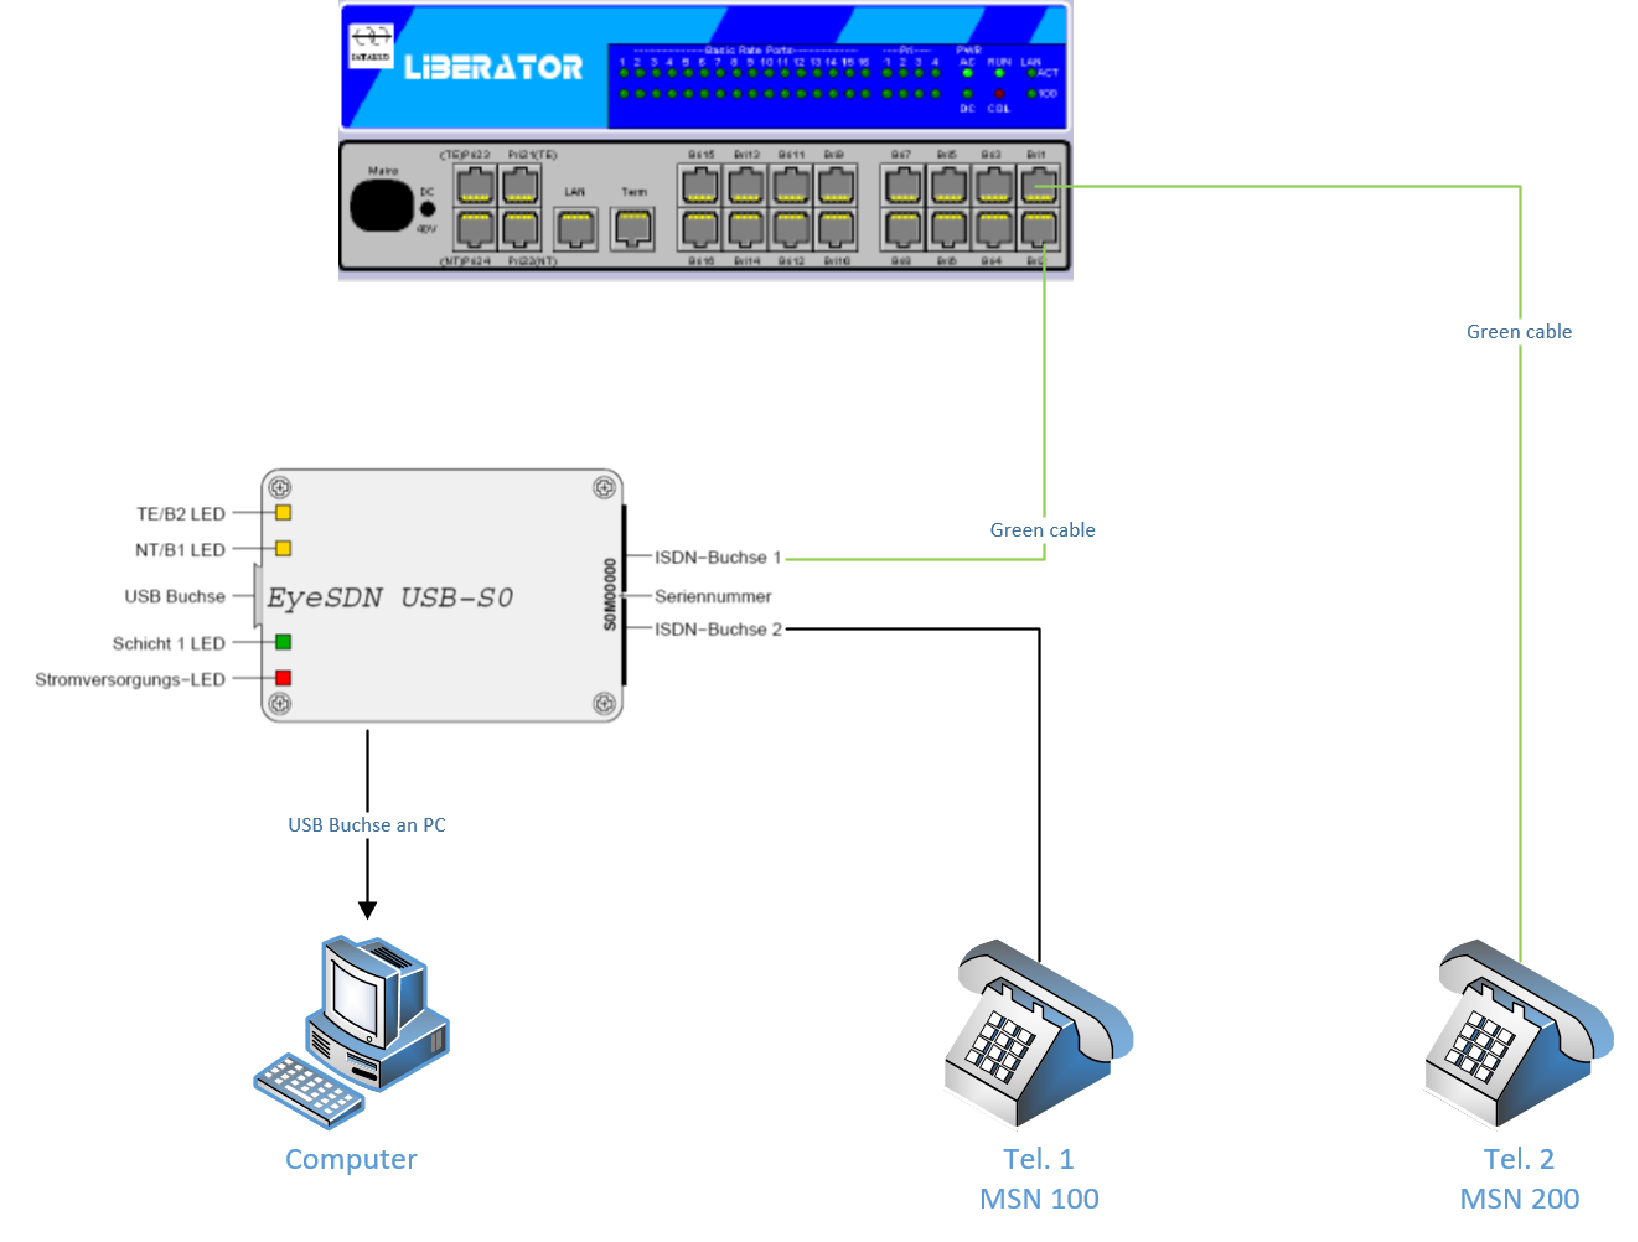
\includegraphics[width=\linewidth]{Graphics/Versuchsaufbau}
\caption{Versuchsaufbau}
\label{fig:versuch}
\end{figure}

\clearpage

\subsection{Komponenten}

\begin{itemize}
  \item Telefon 1 mit der Rufnummer 100
  \item Telefon 2 mit der Rufnummer 200
  \item ISDN Switch Patapsco Liberator S, verbunden mit
  	\begin{itemize}
    \item Verbindung zum EyeSDN USB-S0
    \item Verbindung zum Telefon 2
    \item fungiert als Vermittlungsstelle
	\end{itemize}
  \item EyeSDN USB-S0
  	\begin{itemize}
    \item Verbindung zum Telefon 1
    \item Verbindung zum Computer
    \item schneidet das D-Kanalprotokoll mit
	\end{itemize}
\end{itemize}


\section{Versuchsdurchf�hrung}

Nach dem Versuchsaufbau wird die Anwendung EyeSDN gestartet und sichergestellt,
dass der Mitschnittdienst aktiviert ist. Der Switchmanager wird ebenfalls
gestartet (Login als Super User).\\Im Anschluss wird durch Starten des ISDN Softswitch
Liberator S1 eine Verbindung zum ISDN Switch hergestellt.
Um die Telefone zu aktivieren werden die ISDN BRI Ports 1 und 2 konfiguriert.
Danach wird das Call Routing eingerichtet. Dies geschieht durch Anlegen eines
Routingprofils f�r die Route von Telefon 1 zu Telefon 2 und ein Profil f�r den
umgekehrten Fall.\\In den Profilen werden die entsprechenden Ports aktiviert und
die MSN-Nummer zu den durchgeroutet werden soll, eingetragen.\\Nach den
beschriebenen Kofigurationen wird ein Anruf get�tigt und ein Teilnehmer
beendet den Anruf durch Auflegen. Der Mitschnitt dieses Telefonats wird im
Anschluss mittels des Analysetools Wireshark genauer betrachtet und analysiert.

%Konfiguration erl�utern
%Ports
%mehr auf Routigprofile eingehen

\section{Versuchsziel}

Mit dem beschriebenen Versuchsaufbau soll das Funktionsprinzip
einer Verbindungsauf- und abbauphase innerhalb des Basisanschlusses
veranschaulicht und das D-Kanal-Protokoll einer Telefnverbundung interpretiert
werden. Au�erdem sollen in diesem Zusammenhang die Informationslemente n�her
betrachtet werden. In \label{kap2} folgt die Analyse, die sich an den
Versuchsaufgaben orientiert.
